While the jet mass differential cross section holds great potential for Monte Carlo tuning, it is only one of many. The last several years have produced numerous measurements of jet and jet substructure observables at the LHC. 
Some of these measurements have been motivated by improving parton distribution functions and testing perturbative QCD predictions, 
while others have been designed to improve jet modeling by providing new and better inputs to Monte Carlo tuning.
Some of these, like the fragmentation functions~\cite{Aad:2019onw}, have been used for years to tune Monte Carlo predictions, 
while others, like the Lund Jet Plane~\cite{lundAtlas}, are measurements of observables which have only recently been proposed~\cite{lundPlane}.

With all of these observables, it is useful to consider which measurements are the most constraining for tuning jet modeling.
This is important for motivating future measurements, and can also be used to understand characteristics of the most effective observables.
This study compares several classes of variables in order to provide a more in-depth understanding of the interplay between observables and tuning.
Several simplifications were made in order to ease the comparisons. 
To remove any dependence on topologies, only measurements in dijet events are considered, and only 13 TeV measurements are used.
While both ATLAS and CMS have produced several measurements of jet substructure observables, only ATLAS measurements are considered, since there are more available measurements.

This leaves four measurements which have HepData~\cite{Buckley:2010jn,Maguire:2017ypu} and RIVET~\cite{Buckley:2010ar} routines available.  A list of jet substructure measurements from the LHC can be found at \href{https://twiki.cern.ch/twiki/bin/view/LHCPhysics/LHCJetSubstructureMeasurements}{this twiki}.  Some of the routines for these measurements were prepared at the Les Houches workshop.


These studies scan a similar set of parameters as the ATLAS A14 tune~\cite{ATL-PHYS-PUB-2014-021}, focusing on parameters which are sensitive to parton showers and hadronization.
In addition to parameters which were considered for A14, one additional parameter, \texttt{StringPT:sigma}, is included due to its sensitivity to hadronization.
The list of parameters and their ranges of allowed values are shown in Table~\ref{tab:parameterSpace}.
The parameter space is scanned using a sampling of 300 different configurations determined by PROFESSOR2~\cite{Buckley:2009bj}, and the results are fit with a 3rd order polynomial.
For the soft drop observables (SDO) results, each configuration is run with PYTHIA~8~\cite{Sjostrand:2006za,Sjostrand:2007gs,Sjostrand:2014zea} using a \texttt{PhaseSpace:pTHatMin} of 300 GeV, 
while the other three measurements are run with \texttt{PhaseSpace:pTHatMin} of 400 GeV, each with 200,000 events per configuration. 
This allows sufficient sampling of the parameter space for the specific $p_{T}$ cuts of each analysis. 

\begin{table}[ht!]
\caption{Choices of parameters to tune, and their maximum and minimum values.}
\centering\begin{tabular}{ | c | | c | c | } \hline
                                     & Min. Value   & Max. Value    \\ \hline
\texttt{SigmaProcess:alphaSvalue}             &  0.12        & 0.15    \\ \hline
\texttt{BeamRemnants:primordialKThard}        &  1.5         & 2.0     \\ \hline
\texttt{SpaceShower:pT0Ref}                   &  0.75        & 2.0     \\ \hline
\texttt{SpaceShower:pTmaxFudge}               &  0.5         & 1.5     \\ \hline
\texttt{SpaceShower:pTdampFudge}              &  1.0         & 1.5     \\ \hline
\texttt{SpaceShower:alphaSvalue}              &  0.10        & 0.15    \\ \hline
\texttt{TimeShower:alphaSvalue}               &  0.10        & 0.15    \\ \hline
\texttt{StringPT:sigma}                       &  0.3         & 0.37    \\ \hline
\texttt{MultipartonInteractions:pT0Ref}       &  1.5         & 3.0     \\ \hline
\texttt{MultipartonInteractions:alphaSvalue}  &  0.1         & 0.15    \\ \hline
\end{tabular}
\label{tab:parameterSpace}
\end{table}

Several sets of tunes are compared in order to disentangle different effects from the measurement. In all cases, the results are compraed for four different observables:
the soft drop jet mass distribution for $\beta=0$, the soft drop jet mass distribution for $\beta=2$, the number of subjets in a soft-dropped jet $N_{\mathrm{subjets}}$, and $\mathrm{ECF}_2^{\mathrm{norm}}$.
The two mass measurements provide insight into different aspects of the tune; $\beta=0$ is more sensitive to the perturbative parton shower information, 
while $\beta=2$ is more affected by hadronization. The number of subjets is sensitive to the hard splittings within a jet, and $\mathrm{ECF}_2^{\mathrm{norm}}$ is more sensitive to the 
distribution of energy within the jet. The event and jet selection is defined in the respective papers, and is taken from their RIVET routines.

The first tune comparison studies the sensitivity to the $p_T$ selection and binning used for the measurements. Three different tunes are performed, each using only the jet mass as input.
The first tune uses the three jet mass measurements with different soft drop parameters from Ref.~\cite{softdropMass}, using the inclusive $p_T$ binning. 
The second uses the $p_T$-binned measurements from the same measurement. These two measurements both require that the jet $p_T > 600$ GeV, and so the third uses a new measurement of the
same observable, but with a $p_T$ cut of 300 GeV. This third tune also uses the $p_T$ inclusive measurements only, since the higher $p_T$ bins are poorly populated with the available statistics.
The results of these three tunes are shown in Figure~\ref{massOnlyTune}. 
The two tunes which use the high-$p_T$ measurement produce similar tunes, with similar uncertainties on their parameters. 
While the $p_T$-binned result in principle provides more access to information such as quark-gluon differences or scaling with $p_T$, the impact on the results is small. 
Unlike these, the low-$p_T$ result produces a significantly different tune, despite being the same observable. 
At lower $p_T$, nonperturbative effects become more significant at higher values of $\rho$, while information about the fixed-order and perturbative region is compressed into fewer bins.
This means that it is less able to constrain effects from the parton shower, likely resulting large deviations seen for the soft drop $\beta=2$ jet mass distribution.
While the high-$p_T$ tunes produce better predictions for the jet mass, the low-$p_T$ tune provides a better description of the distribution of soft information within the jet, 
as seen by the better agreement in the number of subjets and $\mathrm{ECF}_2$.


\begin{figure}
\begin{center}
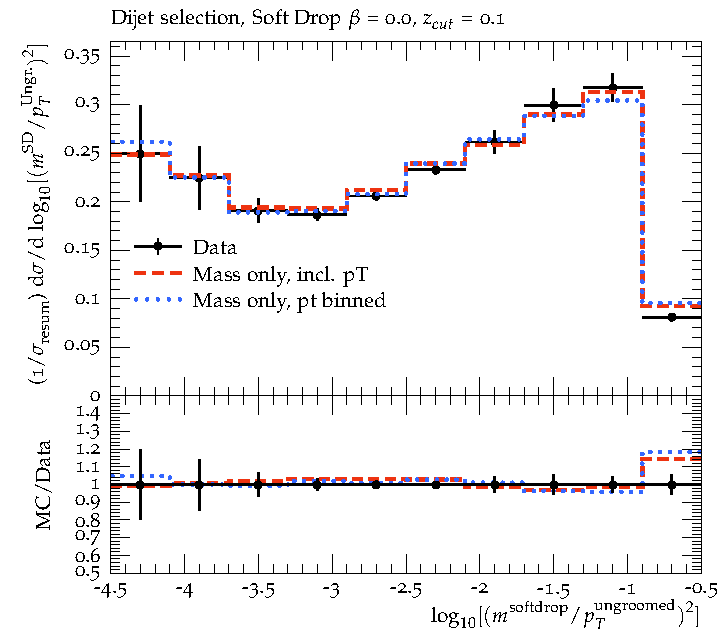
\includegraphics[width=0.49\textwidth]{figs/RivetPlotsMassOnly/SoftDropMass/d01-x01-y01.pdf} \hfill
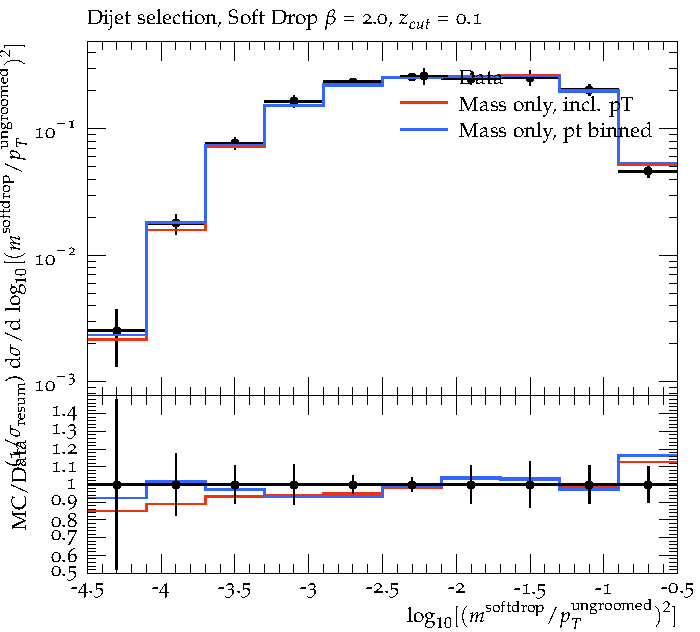
\includegraphics[width=0.49\textwidth]{figs/RivetPlotsMassOnly/SoftDropMass/d03-x01-y01.pdf} \hfill
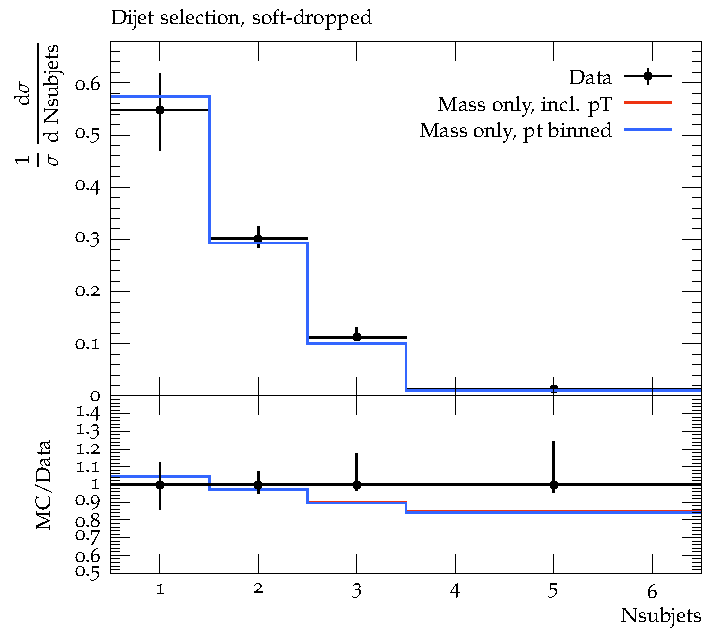
\includegraphics[width=0.49\textwidth]{figs/RivetPlotsMassOnly/ATLAS_2019_I1724098/d23-x01-y01.pdf} \hfill
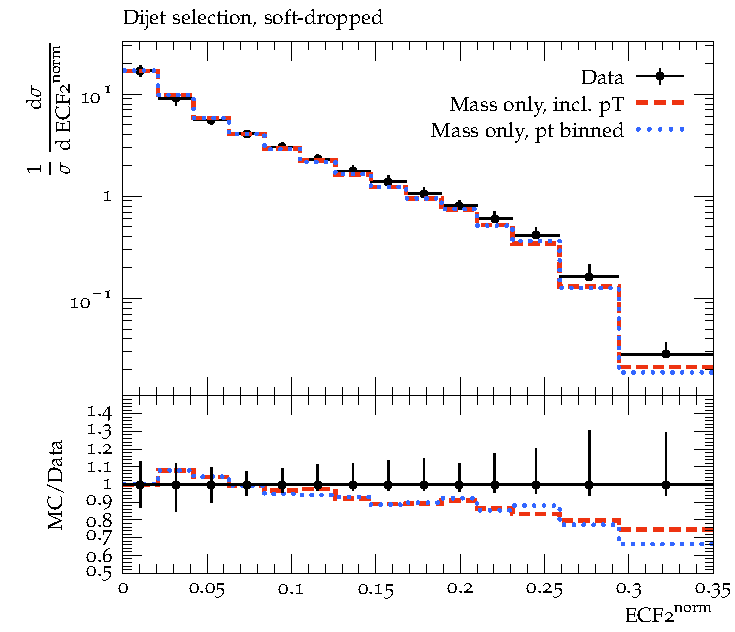
\includegraphics[width=0.49\textwidth]{figs/RivetPlotsMassOnly/ATLAS_2019_I1724098/d27-x01-y01.pdf} \hfill
\end{center}
\label{massOnlyTune}
\end{figure}


The final set of tunes compares the results from each individual measurement. The first of these is the same tune as before, using the $p_T$ inclusive soft drop jet mass measurements at high $p_T$.
The second is the tune using the calorimeter-based measurements of $\rho$, $r_g$, and $z_g$, also inclusive in $p_T$. 
The last tune uses the measurements of several TODO how many jet substructure measurements in jets groomed with the soft drop algorithms, as measured in Ref~\cite{jssObservables}.
These measurements are compared to two standard tunes: the ATLAS A14 tune, and the MONASH tune.
The results of these are shown in Figure~\ref{allTune}. 
A few trends may be seen from these results. In general, the agreement of substructure observables is improved by the use of substructure measurements compared to the ATLAS A14 tune.
As demonstrated in the mass distribution, the tunes from this study seem to lack some information about the fixed-order tune, 
and so they likely need to be combined with other measurements for full accuracy. 
The soft drop jet observables tune is the only tune which accurately reproduces the behavior of $N_{\mathrm{subjets}}$ and $\mathrm{ECF}_2^{\mathrm{norm}}$, though with
degraded agreement for the $\beta=2$ jet mass distribution.


\begin{figure}
\begin{center}
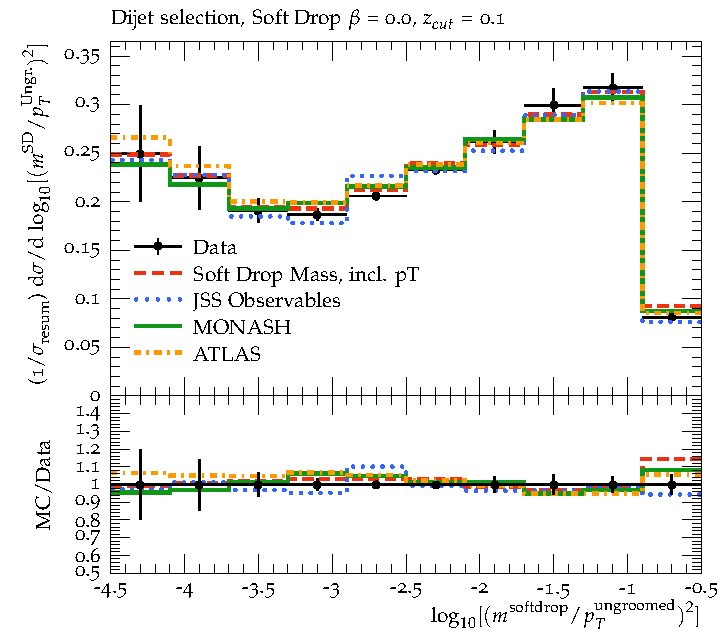
\includegraphics[width=0.49\textwidth]{figs/RivetPlotsFinal/SoftDropMass/d01-x01-y01.pdf} \hfill
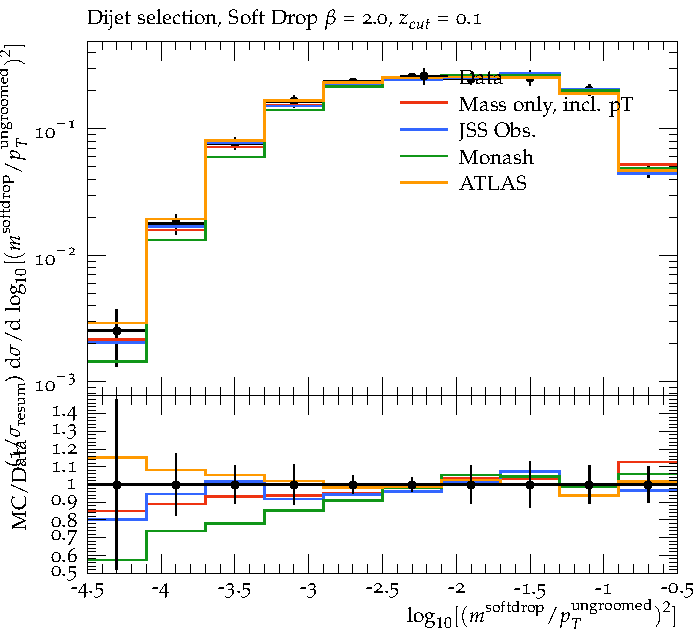
\includegraphics[width=0.49\textwidth]{figs/RivetPlotsFinal/SoftDropMass/d03-x01-y01.pdf} \hfill
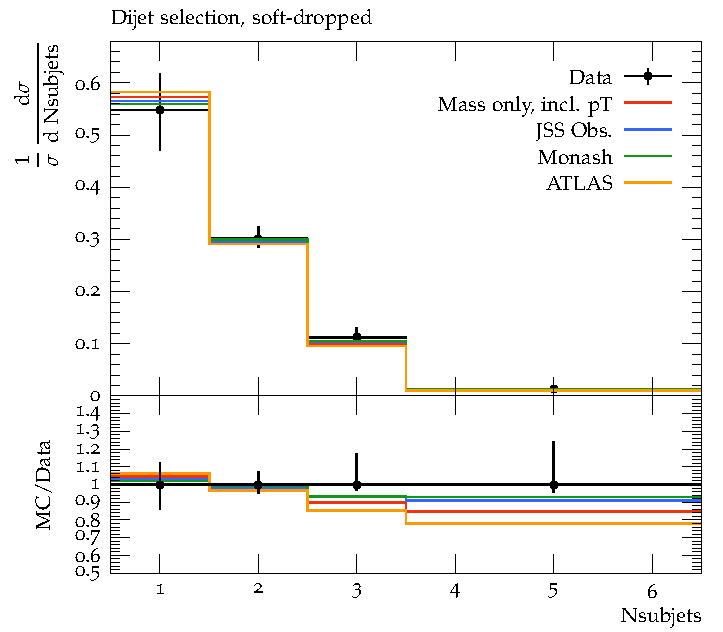
\includegraphics[width=0.49\textwidth]{figs/RivetPlotsFinal/ATLAS_2019_I1724098/d23-x01-y01.pdf} \hfill
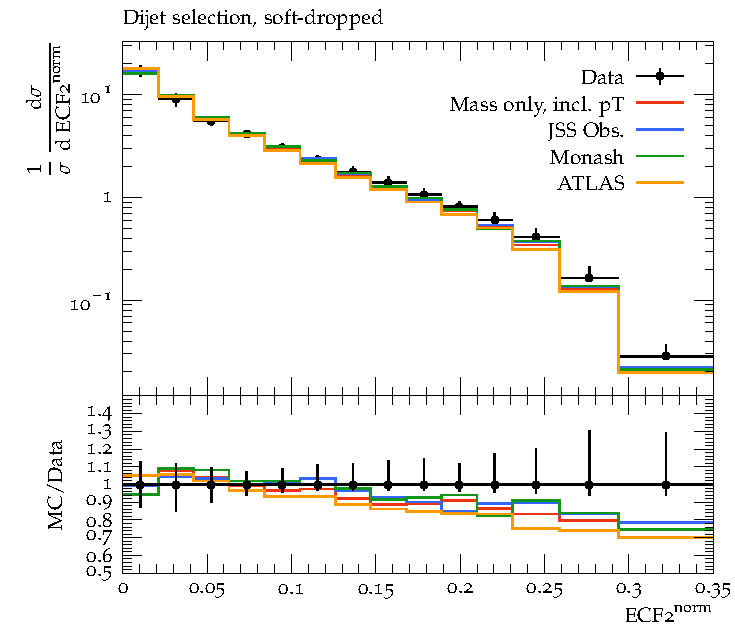
\includegraphics[width=0.49\textwidth]{figs/RivetPlotsFinal/ATLAS_2019_I1724098/d27-x01-y01.pdf} \hfill
\end{center}
\label{allTune}
\end{figure}


The full set of tuned parameters and their uncertainties is shown in Table~\ref{tuneResults}. 
While the agreement of a specific observable typically cannot be linked directly linked to a single tuned parameter, some trends are observed.
Tunes produced from Ref~\cite{softdropObs} tend to have a larger value for TimeShower:alphaSvalue. No other obvious trends can be seen compared to the high-$p_T$ mass tunes, 
indicating that this could be related to the slope seen for the soft drop $\beta=2$ mass distribution.
Tunes produced from Refs~\cite{softdropObs} and ~\cite{jssObs} tend to have higher values of SigmaProcess:alphaSvalue, though both of these measurements are not too sensitive to the hard process.


\clearpage
\begin{landscape}
\begin{table}[ht!]
\caption{Values of tuned parameters.}
\centering\begin{tabular}{ | c | | c | c | c | c | c |} \hline
                                     & MONASH   & ATLAS  & SDM Incl Pt   & SDM Pt Binned & JSS Observables  \\ \hline
SigmaProcess:alphaSvalue             &  0.130   & 0.144  & 0.126+/-0.003 & 0.126+/-0.001 & 0.133+/-0.002 \\ \hline
BeamRemnants:primordialKThard        &  1.8     & 1.72   & 1.825+/-0.055 & 1.794+/-0.011 & 1.785+/-0.048 \\ \hline
SpaceShower:pT0Ref                   &  2.0     & 1.30   & 1.668+/-0.100 & 1.744+/-0.078 & 1.721+/-0.121 \\ \hline
SpaceShower:pTmaxFudge               &          & 0.95   & 1.150+/-0.054 & 1.071+/-0.014 & 1.036+/-0.034 \\ \hline
SpaceShower:pTdampFudge              &          & 1.21   & 1.214+/-0.058 & 1.157+/-0.011 & 1.284+/-0.040 \\ \hline
SpaceShower:alphaSvalue              &  0.1365  & 0.125  & 0.123+/-0.003 & 0.126+/-0.001 & 0.130+/-0.003 \\ \hline
TimeShower:alphaSvalue               &  0.1365  & 0.126  & 0.132+/-0.001 & 0.131+/-0.001 & 0.133+/-0.000 \\ \hline
StringPT:sigma                       &  0.335   &        & 0.348+/-0.003 & 0.350+/-0.003 & 0.333+/-0.006 \\ \hline
MultipartonInteractions:pT0Ref       &  2.28    & 1.98   & 2.000+/-0.100 & 2.181+/-0.049 & 2.441+/-0.148 \\ \hline
MultipartonInteractions:alphaSvalue  &  0.130   & 0118   & 0.116+/-0.003 & 0.126+/-0.002 & 0.128+/-0.003 \\ \hline
\end{tabular}
\label{tab:tuneResults}
\end{table}\end{landscape}
\clearpage



More study is needed in order to fully understand the implications of these results, but there are a few interesting comments. 
The high-$p_T$ soft drop jet mass distribution was designed to study perturbative QCD, but also had several bins sensitive to non-perturbative effects. 
With these preliminary studies, it appears to be as effective in tuning as Ref~\cite{jssObs}, even though it uses fewer observables. 
This is likely due to the factorization of different effects in the soft drop mass distribution, allowing it to be simultaneously sensitive to fixed order effects, the parton shower, and hadronization. 
This shows that factorization is important, and that it is important to be sensitive to a variety of effects when creating these tunes.







